\documentclass[border=6pt]{standalone}
\usepackage{tikz}
\usetikzlibrary{arrows.meta,calc,decorations.pathreplacing}
\begin{document}
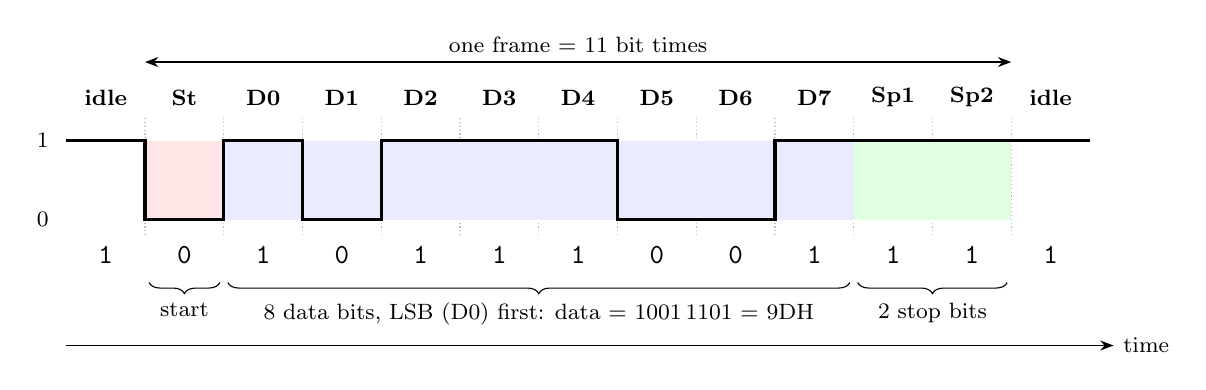
\begin{tikzpicture}[>=Stealth,font=\small,x=1.0cm,y=1cm]
% bit cells: idle, St, D0..D7, Sp1, Sp2, idle
\def\names{{"idle","St","D0","D1","D2","D3","D4","D5","D6","D7","Sp1","Sp2","idle"}}
\def\bits{{1,0,1,0,1,1,1,0,0,1,1,1,1}}
\foreach \i in {0,...,12} {
  \pgfmathsetmacro{\n}{\names[\i]}
  \pgfmathtruncatemacro{\b}{\bits[\i]}
  \node[font=\footnotesize\bfseries] at (\i+0.5,1.55) {\n};
  \node[font=\ttfamily] at (\i+0.5,-0.45) {\b};
}
% grid lines at bit boundaries of the frame
\foreach \x in {1,...,12} \draw[gray!50,densely dotted] (\x,-0.2) -- (\x,1.3);
% shading of the frame fields
\fill[red!10] (1,0) rectangle (2,1);
\fill[blue!8] (2,0) rectangle (10,1);
\fill[green!12] (10,0) rectangle (12,1);
% waveform (high = 1)
\draw[very thick] (0,1) -- (1,1) -- (1,0) -- (2,0) -- (2,1) -- (3,1) -- (3,0) -- (4,0) -- (4,1)
  -- (7,1) -- (7,0) -- (9,0) -- (9,1) -- (13,1);
\node[anchor=east,font=\footnotesize] at (-0.1,1) {1};
\node[anchor=east,font=\footnotesize] at (-0.1,0) {0};
% field braces
\draw[decorate,decoration={brace,mirror,amplitude=4pt}] (1.05,-0.8) -- (1.95,-0.8) node[midway,below=4pt,font=\footnotesize]{start};
\draw[decorate,decoration={brace,mirror,amplitude=4pt}] (2.05,-0.8) -- (9.95,-0.8) node[midway,below=4pt,font=\footnotesize]{8 data bits, LSB (D0) first: data = 1001\,1101 = 9DH};
\draw[decorate,decoration={brace,mirror,amplitude=4pt}] (10.05,-0.8) -- (11.95,-0.8) node[midway,below=4pt,font=\footnotesize]{2 stop bits};
\draw[<->] (1,2.0) -- (12,2.0) node[midway,above,font=\footnotesize]{one frame = 11 bit times};
\draw[->] (0,-1.6) -- (13.3,-1.6) node[right,font=\footnotesize]{time};
\end{tikzpicture}
\end{document}
